\documentclass[border=5pt]{standalone}
\usepackage{tikz}
\usetikzlibrary{calc}
\usepackage{amsmath}
\begin{document}
        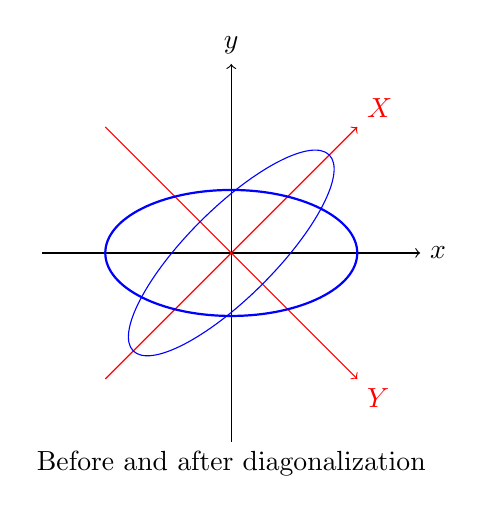
\begin{tikzpicture}[scale=0.8]
            % Original axes
            \draw[->] (-3,0) -- (3,0) node[right] {$x$};
            \draw[->] (0,-3) -- (0,3) node[above] {$y$};

            % Rotated axes
            \draw[red,->] (-2,-2) -- (2,2) node[above right] {$X$};
            \draw[red,->] (-2,2) -- (2,-2) node[below right] {$Y$};

            % Draw ellipse
            \draw[blue, thick] (0,0) ellipse (2cm and 1cm);
            \draw[blue, rotate=45] (0,0) ellipse (2.2cm and 0.7cm);

            % Add explanation
            \node[below] at (0,-3) {Before and after diagonalization};
        \end{tikzpicture}
\end{document}
